\chapter{Wariancja Allana}\label{chap:appx:allan}
Wariancja Allana jest metodą wykorzystywaną do określenia charakterystyk szumów zawartych w~sygnałach mierzonych przez układy oparte o~oscylatory. Metoda ta została opisana w~\cite{Allan1966} jako część pracy magisterskiej w~latach 60-tych XX wieku i~od tamtego czasu została przyjęta jako standardowa do wyznaczania charakterystyk tego typu układów. W~literaturze można znaleźć między innymi prace opisujące analizę sygnałów układów inercyjnych \cite{El-Sheimy2008, FreescaleSemiconductor2015}, czy układów GPS \cite{Wright2007}. 
Wariancja Allana ($\sigma^2(\tau)$) wyznaczana jest dla sygnału $\Omega$ wyrażonego w~domenie czasu i~podzielonego na $n$ klastrów o~czasie trwania $\tau$ każdy. Przyjmując, że $K$ oznacza numer klastra badanego sygnału znajdujący się w~chwili czasu [$K\tau_0 , K\tau_0+\tau$], wariancję Allana możemy wyrazić za pomocą równań \ref{eq:appx:allan:clusterAverage} i~\ref{eq:appx:allan:avar}:
\begin{equation}
	\label{eq:appx:allan:clusterAverage}
	\overline{\Omega}_K(\tau) = \frac{1}{\tau}\int_{K_{\tau_0}}^{K_{\tau_0}+\tau}\Omega(t)dt
\end{equation}
\begin{equation}
	\label{eq:appx:allan:avar}
	\sigma^2(\tau) = \frac{1}{2(N-2n)}\sum_{K=1}^{N-2n}[\overline{\Omega}_{K+1}(\tau)-\overline{\Omega}_K(\tau)]^2
\end{equation}

\begin{figure}[H]
	\centering
	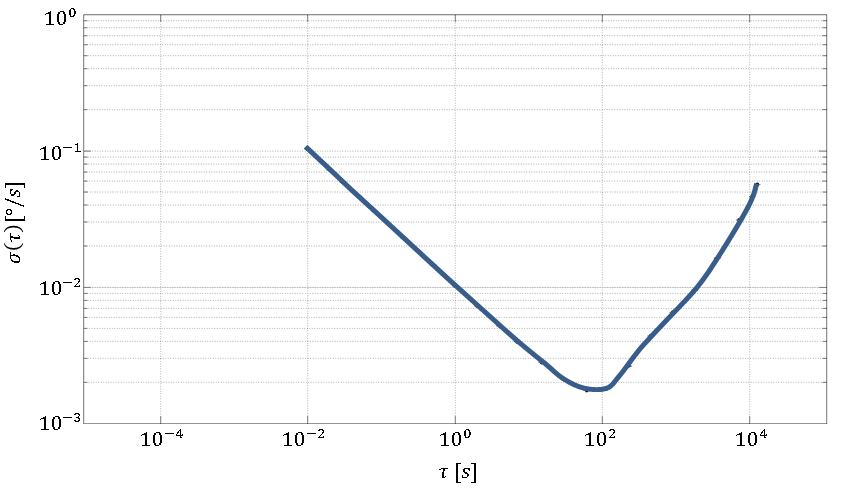
\includegraphics[width=0.7\textwidth]{images/Allans2GyroXosig.png}
	\caption{Wykres funkcji odchylenia Allana dla sygnału osi X żyroskopu}
	\label{fig:appx:allan:deviationPlot}
\end{figure}

Aby na podstawie wyznaczonej wariancji określić charakterystyki szumów należy obliczyć odchylenie Allana $\sigma(\tau) = \sqrt{\sigma^2(\tau)}$ i~przeanalizować przebieg tej funkcji na wykresie w~skali logarytmicznej (przykładowy wykres odchylania Allana dla żyroskopu przedstawia wykres z rysunku \ref{fig:appx:allan:deviationPlot}). Wykres ten zawiera informacje o~5 różnych rodzajach szumu jaki zawarty jest w~badanym sygnale:

\begin{enumerate}
	\item {\emph{Quantization noise} -- szum wprowadzony w~trakcie konwersji sygnału analogowego na cyfrowy i~spowodowany przez różnice pomiędzy faktyczną wartością sygnału, a~wartością wynikającą z~punktu, w~którym nastąpiło próbkowanie.}
	\item {\emph{Angle (velocity) random walk} -- szum wysokiej częstotliwości obserwowalny nawet w~czasie krótkich pomiarów. Jego występowanie znacząco obniża dokładność prowadzonych obliczeń.}
	\item {\emph{Bias instability} -- szum niskiej częstotliwości związany ze zmianą właściwości fizycznych materiałów, z~których zbudowane są czujniki, a~przez to niepoprawną interpretacją napięcia elektrycznego działającego w~urządzeniu.}
	\item {\emph{Rate random walk} -- szum wysokiej częstotliwości pojawiający się w~pomiarach w~dłuższym okresie czasu. Jego pochodzenie nie jest do końca znane.}
	\item {\emph{Rate ramp} -- systematycznie pojawiający się błąd pomiarów, którego wartość zależna jest od czasu działania. Pomiary zakłócone tego rodzaju szumem nie są w~stanie powrócić do wartości początkowych.}	
\end{enumerate}

Powyższe zakłócenia pomiarów zawarte są na wykresie odchylenia jako obszary, w~których kąt nachylenia wykresu do osi $X$ jest zbliżony do kąta nachylenia prostej o~współczynniku kierunkowym $\alpha$ wynoszącym odpowiednio: $-1, -0.5, 0, 0.5 , 1$. Obszary te są widoczne na wykresie z rysunku \ref{fig:appx:allan:slopes}.
\begin{figure}[H]
	\centering
	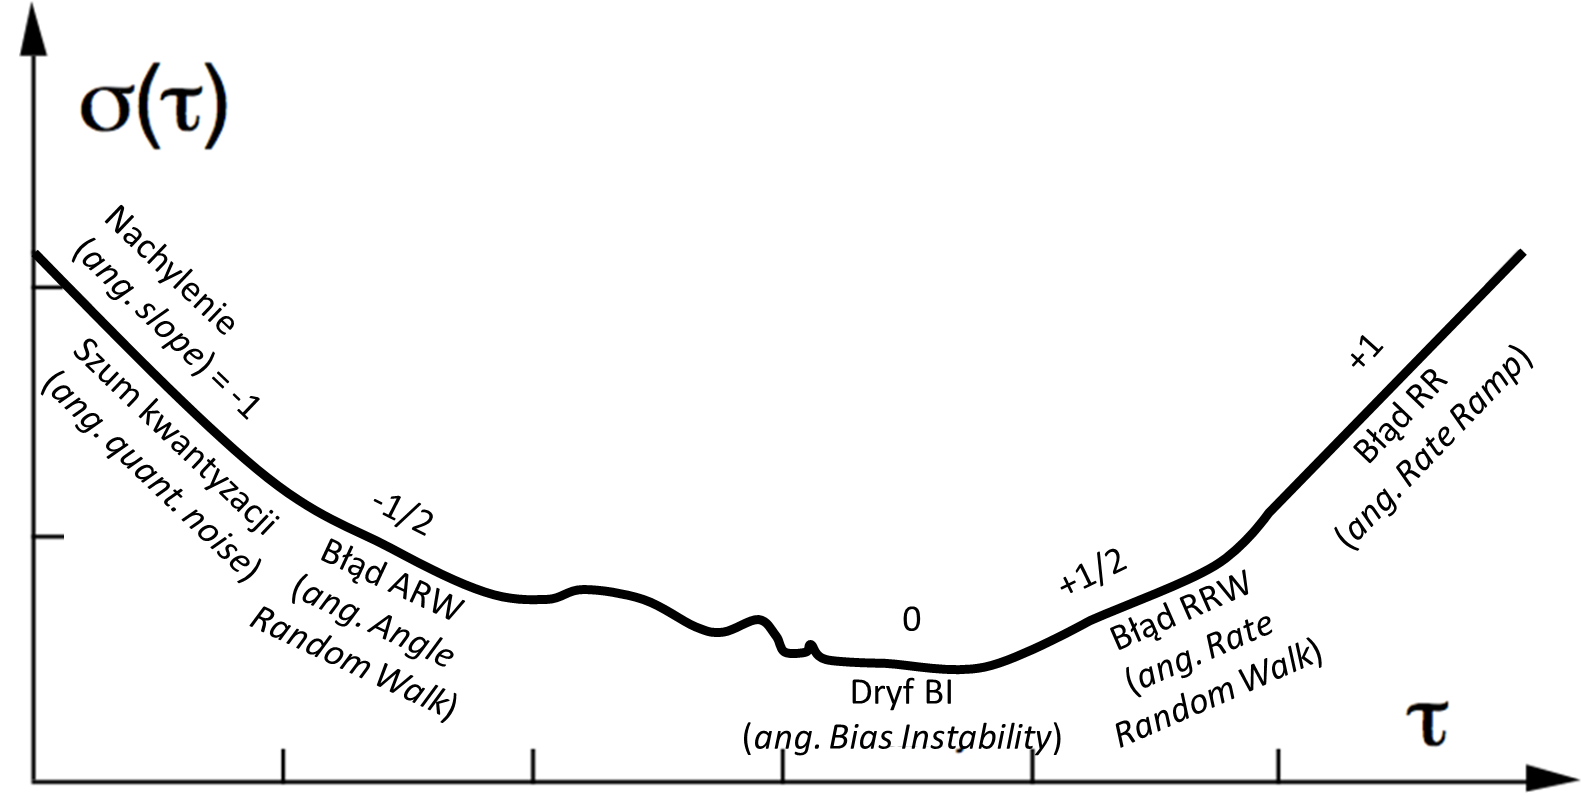
\includegraphics[width=0.6\textwidth]{images/slopes.png}
	\caption{Obszary szumów na wykresie odchylenia Allana \autocite{s120202219}}
	\label{fig:appx:allan:slopes}
\end{figure}

Nie zawsze wykres funkcji $\sigma(\tau)$ musi zawierać wszystkie 5 obszarów co oznacza, że niektóre rodzaje szumów mogą nie występować.